\documentclass[12pt, titlepage]{article}

\usepackage{booktabs}
\usepackage{tabularx}
\usepackage{hyperref}
\usepackage{pdflscape}
\usepackage{graphicx}
\usepackage{float}
\hypersetup{
    colorlinks,
    citecolor=blue,
    filecolor=black,
    linkcolor=red,
    urlcolor=blue
}
\usepackage[round]{natbib}

%% Comments

\usepackage{color}

\newif\ifcomments\commentstrue %displays comments
%\newif\ifcomments\commentsfalse %so that comments do not display

\ifcomments
\newcommand{\authornote}[3]{\textcolor{#1}{[#3 ---#2]}}
\newcommand{\todo}[1]{\textcolor{red}{[TODO: #1]}}
\else
\newcommand{\authornote}[3]{}
\newcommand{\todo}[1]{}
\fi

\newcommand{\wss}[1]{\authornote{blue}{SS}{#1}} 
\newcommand{\plt}[1]{\authornote{magenta}{TPLT}{#1}} %For explanation of the template
\newcommand{\an}[1]{\authornote{cyan}{Author}{#1}}

%% Common Parts

\newcommand{\progname}{ProgName} % PUT YOUR PROGRAM NAME HERE
\newcommand{\authname}{Team \#, Team Name
\\ Student 1 name
\\ Student 2 name
\\ Student 3 name
\\ Student 4 name} % AUTHOR NAMES                  

\usepackage{hyperref}
    \hypersetup{colorlinks=true, linkcolor=blue, citecolor=blue, filecolor=blue,
                urlcolor=blue, unicode=false}
    \urlstyle{same}
                                


\begin{document}

\title{System Verification and Validation Plan for \progname{}} 
\author{\authname}
\date{\today}
	
\maketitle

\pagenumbering{roman}

\section*{Revision History}

\begin{tabularx}{\textwidth}{p{3cm}p{2cm}X}
\toprule {\bf Date} & {\bf Version} & {\bf Notes}\\
\midrule
2025-02-27 & 1.0 & Initial Release\\
\bottomrule
\end{tabularx}

\newpage

\tableofcontents
\listoftables

\listoffigures

\newpage
\section{Symbols, Abbreviations, and Acronyms}

\renewcommand{\arraystretch}{1.2}
\begin{tabular}{l l} 
  \toprule		
  \textbf{symbol} & \textbf{description}\\
  \midrule
  CAS & Computing and Software\\
  CI & Continuous Integration\\
  DE & Domain Expert \\
  $d_{total}$ & bin size, or number of binary descriptions \\
  $D_{bin}$ & 1D array of 32 byte binary strings \\
  FOV & field-of-view\\
  $I$ & 2D array of pixel values for a greyscale image \\
  $I'$ & transformed 2D array of pixel values\\
  $k$ & number of total keypoints\\
  LD & Lead Developer \\
  $m$ & horizontal image dimension\\
  MG & Module Guide \\
  MIS & Module Interface Specification\\
  $n$ & vertical image dimension\\
  ORB & Oriented FAST and Rotated BRIEF\\
  PEP8 & Python Enhancement Proposal-8\\
  PS & Project Supervisor\\
  RGB & Red-Green-Blue coloured imagery\\
  $s$ & patch size\\
  SDI & Software Design Instructor\\
  SLAM & Simultaneous Localization and Mapping\\
  SRS & Software Requirements Specification\\
  $t$ & intensity threshold \\
  VnV & Verification and Validation\\
  $\sigma$ & standard deviation\\
  \bottomrule
\end{tabular}\\

\newpage

\pagenumbering{arabic}
\noindent The intent of this document is to define the verification and validation (VnV) processes
that will be used to assess \progname, (IFC) software. Specifically, this document will be used to 
characterize the behaviour and performance of this software. The remaining sections of this document 
outline a detailed summary of the specific objectives of the VnV campaign. This includes considerations 
for the scope of the VnV efforts with respect to contraints that stem from the CAS 741 
development schedule, as well as anticipated activities beyond the scope of CAS 741.
Verification procedures are present for select deliverables and milestone, and include 
an overview of anticipated cases for both system tests unit tests.

\section{General Information}

\subsection{Summary}
The Image Feature Correspondences (IFC) software is a feature comparison algorithm that is intended 
to be used as part of a pipeline to perform extrinsic camera calibration for 
applications in mobile robotics. It accepts camera configuration parameters and greyscale imagery data at 
different poses to identify common features amongst collected images. 

\subsection{Objectives}
The VnV process is intended to characterize how well the for the IFC software performs in its 
intended capacity to identify features amongst collected imagery. The performance of this system 
can vary significantly as it is influenced by factors such as overlap in camera fields-of-view (FOV),
the observed contrast between objects in an image, and variance in scale, rotation, and ambient 
illumination conditions. Furthermore, as there is no common baseline to compare this software to as 
an oracle, the VnV campaign for the IFC software is intended to characterize the performance of the 
integrated image processing functions against a set of test datasets. Key objectives of this process 
are defined below.

\begin{itemize}
  \item assess the reliability in the feature matching pipeline
  \item assess how users perceive their interactions with the IFC software 
  \item characterize the performances of the IFC software with metrics such as processing time and 
  memory usage
  \item cross-validate the performance of the IFC software with accepted benchmarked datasets
\end{itemize}

Verification of the individual functions within the OpenCV library themselves falls outside of the 
scope of this project, as we can assume that the library has been verified by its own 
implementation team. 
\\ \\

\subsection{Challenge Level and Extras}
The proposed software will serve as the front end of a robust optimization framework 
for extrinsic camera calibration. The IFC software must be capable of handling large volumes of 
high-resolution imagery while ensuring reliability through consistent and repeatable outputs. 
The software will be designed for robustness in data processing, accommodating a wide range of 
input conditions. Additionally, it will maintain a streamlined user experience, allowing users 
to override select default parameters while ensuring that the learning curve remains minimal 
for efficient adoption. 

As the long-term goal for this software is to absorb it into a larger calibration 
pipeline for research in the domain of mobile robotic, this project is defined as 
an advanced level of challenge. In addition to the standard codebase, verification 
report, and documentation for the CAS 741 deliverables, a User Manual shall also be 
submitted to support future development of the IFC software and its integration into 
the full camera calibration pipeline.

\subsection{Relevant Documentation}
Relevant documentation has been hyperlinked throughout the length of the document. This enables 
the reader to access each resource within the context of the section that the reference is 
invoked.

\section{Plan}
This section outlines how each aspect of the VnV effort will be performed. This may be handled by 
milestone or by general practices, such as continuous integration and linters. 

\subsection{Verification and Validation Team}
The VnV team consists of four members, each of whom play a distinct role in the 
verification process. These roles and responsibilities are outlined in Table \ref{Table_Ver_Roles}.

\begin{table}[tbp!]
  \centering
  \begin{tabular}{|p{0.11\linewidth}|p{0.24\linewidth}|p{0.6\linewidth}|} 
    \hline
    \textbf{Name} & \textbf{Role} & \textbf{Description}\\
    \hline
    Kiran Singh & Lead Developer and Test Designer (LD) & Responsibilities include the
    identification of critical business cases for integrated tests, assessment of 
    schedule and scope considerations,  design and implementation of unit tests, 
    system tests, and documentation of test results.\\
    \hline
    Matthew Giamou & Project Supervisor (PS) & Lead consultant on integrated 
    performance needs and decomposition for software modules. Responsibilities 
    include review of proposed VnV scope, as proposed by 
    Kiran S., and provision of feedback to the general scope of the VnV campaign, and approval 
    of the individual test cases that are proposed by the LD. \\
    \hline
    Aliyah Jimoh & Domain Expert (DE) & Responsibilities include provision of 
    feedback on proposed test cases for the 
    scope of test cases for both the functional and non-functional requirements. They 
    will also provide feedback on the code walkthrough per the final CAS 741 presentation. 
    This statisfies the need for a reviewer that is removed from the design effort yet
    still holds sufficient domain knowledge to provide feedback on the overall design 
    and associated VnV efforts.\\ 
    \hline
    Spencer Smith & Software Development Instructor (SDI) & Responsibilities include 
    provision of feedback on proposed test cases for the scope of test cases 
    for both the functional and non-functional requirements. They will also 
    provide feedback on the code walkthrough per the final CAS 741 presentation. 
    This reviewer provides an essential stream of feedback as they are fully removed 
    from the application domain and may willing to question assumptions and address biases 
    that may be implicit amongst other members of the VnV team.\\
    \bottomrule
  \end{tabular}\\
  \caption{Roles and Responsibilities of the Verification and Validation Team}
  \label{Table_Ver_Roles}
\end{table}


\subsection{SRS Verification Plan}
The \textbf{\href{https://github.com/KiranSingh15/CAS-741-Image-Correspondences/blob/main/docs/SRS/SRS.pdf}
{SRS}} shall be reviewed by each member of the reviewer team to form consensus that the SRS has been correctly 
decomposed into sufficient requirements.
\begin{itemize}
\item the models are deemed to be comprehensible
\item the models are deemed to be correct
\item the associated requirements are traced correctly with respect to the models 
and project scope 
\item the requirements are decomposed in a manner that facilitates verification
\end{itemize}
Feedback on the \textbf{\href{https://github.com/KiranSingh15/CAS-741-Image-Correspondences/blob/main/docs/SRS/SRS.pdf}
{SRS}}
 from the DE and SDI will be captured through 
the use of Github Issues. Specifically, both reviewers will use the 
\textbf{\href{https://github.com/KiranSingh15/CAS-741-Image-Correspondences/blob/
main/docs/Checklists/SRS-Checklist.pdf}
{SRS Checklist}}. 
The lead developer will respond in turn to each issue and if 
reserves the right to reject a proposed change as needed. \\
The Lead Developer will schedule a meeting with the PS to walk through 
the first revision of the \textbf{\href{https://github.com/KiranSingh15/CAS-741-Image-Correspondences/blob/main/docs/SRS/SRS.pdf}
{SRS}}
 document. In this meeting, the PS will offer 
feedback and recommendations for candidate revisions to the outlined models and requirements. 
The Lead Developer will then create issues in Github to address each proposed revision.

\subsection{Design Verification Plan}
The DE and SDI will review the Module Guide 
\textbf{\href{https://github.com/KiranSingh15/CAS-741-Image-Correspondences/blob/main/docs/Design/SoftArchitecture/MG.pdf}
{(MG)}} and the Module Interface Specification 
\textbf{\href{https://github.com/KiranSingh15/CAS-741-Image-Correspondences/blob/main/docs/Design/SoftDetailedDes/MIS.pdf}
{(MIS)}} against the 
\textbf{\href{https://github.com/KiranSingh15/CAS-741-Image-Correspondences/blob/main/docs/Checklists/MG-Checklist.pdf}
{MG}} and
\textbf{\href{https://github.com/KiranSingh15/CAS-741-Image-Correspondences/blob/main/docs/Checklists/MIS-Checklist.pdf}
{MIS}} checklists. The objective of this review cycle is to ensure that the design of the system:
\begin{enumerate}
\item is unambiguous
\item adheres to best-practices of module design
\item aligns with the requirements as identified in the 
\textbf{\href{https://github.com/KiranSingh15/CAS-741-Image-Correspondences/blob/main/docs/SRS/SRS.pdf}
{SRS}}
\end{enumerate}


\subsection{Verification and Validation Plan Verification Plan}
The VnV Plan will be verified via inspection by the DE and the 
Software Development Instructor. The 
\textbf{\href{https://github.com/KiranSingh15/CAS-741-Image-Correspondences/blob/main/docs/Checklists/SRS-Checklist.pdf}
{VnV Plan Checklist}} 
will be used as the assessment criteria for the inspection. 
Feedback will provided as Github issues and will be handled in the same manner as feedback 
for the SRS.\\ \\
Mutation testing will be performed against the tests outlined in Section \ref{UTD}, which are expected to be 
completed as part of a Rev 2.0 release of the VnV Plan, as part of the initial release (Rev 1.0) of the 
{\href{https://github.com/KiranSingh15/CAS-741-Image-Correspondences/blob/main/docs/Design/SoftArchitecture/MG.pdf}
{(MG)}} and 
{\href{https://github.com/KiranSingh15/CAS-741-Image-Correspondences/blob/main/docs/Design/SoftDetailedDes/MIS.pdf}
{(MIS)}}.

\subsection{Implementation Verification Plan}
The IFC software shall be verified against the test procedures outlined in Sections \ref{FR_Tests} and 
\ref{NFR_Tests}. Static verification of the IFC software will consist of a code walkthrough. This will take 
place during the CAS 741 final presentation, where the DE and SDI will have the opportunity to observe 
the code and raise issues following the presentation via GitHub. \\ \\
Dynamic verification of the IFC software will consist of system and unit tests via PyTest. System tests 
are outlined in Section \ref{Sys_Tests}. Unit tests will be outlined in Rev 2 of the VnV Plan in 
Section \ref{UTD}.

\subsection{Automated Testing and Verification Tools}
Several tools will be used to support automated testing and verification. They include:
\begin{itemize}
\item Continuous Integration (CI) will be facilitated via GitHub Actions. A pull request will be used 
to run automated tests.
\item Pytest will be used to execute system tests, unit tests, and to assess code coverage. 
\item flake8 will be used as a linter to ensure adherence to PEP8 standards. 
\item PyLint, as an alternative linter to flake8.
\end{itemize}

\subsection{Software Validation Plan}
The IFC software will be compared against benchmark data from one or more of the following 
\href{https://github.com/youngguncho/awesome-slam-datasets}{SLAM datasets} that feature camera imagery data. 
These datasets provide a much more challenging scene to identify and match features than generated binary markers. 
Imagery from the selected datasets will be preprocessed 
from RGB data to greyscale data, and will undergo a testing procedure similar to that of the systems tests 
outlined in Section \ref{FR_Tests}. These tests would be inclusive of the general form of timing and memory 
usage  metrics outlined in Section \ref{Performance}. These tests may exceed the constraints of the  CAS 
741 schedule and will be continued as part of future work.

\section{System Tests}\label{Sys_Tests}
This section outlines the general roadmap for the required integrated system tests. 
\subsection{Tests for Functional Requirements} \label{FR_Tests}
This section outlines the system tests that verify the requirements outlined in 
Section 5 of the 
\textbf{\href{https://github.com/KiranSingh15/CAS-741-Image-Correspondences/blob/main/docs/SRS/SRS.pdf}
{SRS}}. 

\begin{figure}[h!]
  \begin{center}
   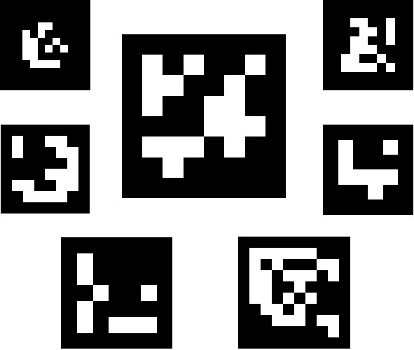
\includegraphics[width=0.6\textwidth]{images/ArUco_Field_Gen.jpg}
  \caption[An example of a generated ArUco pattern]{An example of a generated ArUco pattern. Image taken 
  from \cite{ARUCO_Markers_openCV}}
  \label{gen_aruco} 
  \end{center}
\end{figure}

\begin{figure}[h!]
  \begin{center}
   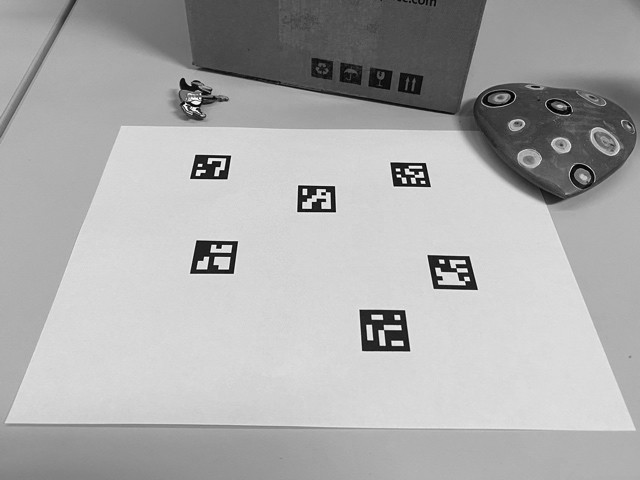
\includegraphics[width=0.6\textwidth]{images/GS_ArUco_Field_Image.jpg}
  \caption[An example of ArUco patterns within the scene of a captured greyscale image]
  {An example of ArUco patterns within the scene of a captured greyscale image. 
  Image taken from \cite{ARUCO_Markers_openCV}}
  \label{gs_aruco_field} 
  \end{center}
\end{figure}

\subsubsection{Feature Detection}
This test section is intended to assess that the system can accept new parameters from users and covers 
requirements R1 through R7 and R9 through R11, in Section 5.1 of the 
\textbf{\href{https://github.com/KiranSingh15/CAS-741-Image-Correspondences/blob/main/docs/SRS/SRS.pdf}
{SRS}}. 
		
\paragraph{Image Smoother}
\begin{enumerate}
\item \hypertarget{STFR-IS-01}{\textbf{STFR-IS-01}}

\textbf{Requirements Addressed:} R1, R5, R9

\textbf{Control:} Automated		

\textbf{Initial State:} Uninitialized

\textbf{Input:} Generated binary patterned fiducial markers, named 
\href{https://docs.opencv.org/4.x/d5/dae/tutorial_aruco_detection.html}
{ArUco} markers, will be used as simplified targets for corner detection. A depiction of these markers is shown 
in Figure \ref{gen_aruco}. A collection of 20 images that contain ArUco markers within the image scene will be 
provided as test inputs, as shown in Figure \ref{gs_aruco_field}. Each image $I$ will be defined as 2D array of 
a user-specified resolution. The user will also assign the image intensity standard deviation $\sigma$ to define 
the size of the Gaussian Kernel.

\textbf{Output:} 20 output images as a 2D array, each of which have a descriptive name that clearly identifies the 
input image from which it originates. The $I'$ array should be of equal size and the same data type as its 
corresponding image $I$. All images should be saved under its own uniquely named folder to prevent mixing 
of input and output imagery.

\textbf{How test will be performed:} Automated Tools (i.e. Pytest)

\end{enumerate}


\paragraph{Keypoint Detector}
\begin{enumerate}
\item \hypertarget{STFR-KP-01}{\textbf{STFR-KP-01}\\}
\textbf{Requirements Addressed:} R2, R6, R10

\textbf{Control:} Automatic	

\textbf{Initial State:} Uninitialized			

\textbf{Input:} A collection of 20 smoothed images $I'$, each defined as 2D array of specified resolution, that 
contain a binary patterned fiducial markers as outlined in System Test \hyperlink{STFR-IS-01}{STFR-IS-01}. 
A permissible image intensity threshold, $t$, shall also be introduced, where $t$ is defined as a non-zero 
positive integer between 1 and 255.

\textbf{Output:} A flag which indicates that corner detection is active. 
A 2D array of size ${k \times 2}$, where $k$ is the quantity of identified keypoints, 
where the first and second columns are populated with the horizontal and vertical coordinates for each 
keypoint. Each entry in the array should be an positive integer value. Each array should have a unique identifier that 
clearly defines the original image from which its keypoints were identified. All output arrays should be saved 
to a unique folder to separate them from the input images.

\textbf{How test will be performed:} Automated Tools (i.e. Pytest)
\end{enumerate}

\paragraph{Feature Definition}
\begin{enumerate}
\item \hypertarget{STFR-FD-01}{\textbf{STFR-FD-01}\\}
\textbf{Requirements Addressed:} R3, R4, R7, R11

\textbf{Control:} Automatic

\textbf{Initial State:} Uninitialized

\textbf{Input:} A collection of 20 images, each defined as a 2D array of integers, and a collection of 20 
$k\times 2$ 2D arrays, where $k$ is the number of keypoints within each image. A patch size, $s$, 
will also be input as a scalar integer to define the the region for which to search for descriptors. A target 
number of descriptors titled $d_{total}$, also known as the bin size, will also be provided as a non-negative integer 
between 1 and 1023.

\textbf{Output:} $D_{bin}$, a 1D array of length $d_{total}$ where all entries of the array are 32 byte binary strings. 

\textbf{Test Case Derivation:} \href{https://sites.cc.gatech.edu/classes/AY2024/cs4475_summer/images/ORB_an_efficient_alternative_to_SIFT_or_SURF.pdf}
{ORB: An efficient alternative to SIFT or SURF}. This publication outlines methods 
to develop and the corresponding assessment of binary feature descriptors.

\textbf{How test will be performed:} Automated Tools (i.e. Pytest)
\end{enumerate}

\subsubsection{Feature Comparison}

This test section is intended to assess that the system can accept new parameters from users. It addresses 
requirements R8 and R12 through R15 in Section 5.1 of the 
\textbf{\href{https://github.com/KiranSingh15/CAS-741-Image-Correspondences/blob/main/docs/SRS/SRS.pdf}
{SRS}}. 
		
\paragraph{Descriptor Comparison}
\begin{enumerate}
\item \hypertarget{STFR-DC-01}{\textbf{STFR-DC-01}\\}
\textbf{Requirements Addressed:} R8, R12, R13, R14, R15

\textbf{Control:} Automated		

\textbf{Initial State:} Uninitialized

\textbf{Input:} 20 1D arrays, each which have a unique length, $D_{bin}$, where each element of the 
array is a 32 byte binary string known as a binary descriptor. Each array should be labeled with a 
descriptive name that clearly references the instance of both the camera and pose at the time of image 
capture.

\textbf{Output:} A flag that indicates that Hamming Distances were compared. 
A dynamically-sized array, stored as a Pandas dataframe, where the length of the array is the 
number of matched features. The columns of the array will include the properties as follows.
\begin{itemize}
\item Binary descriptors of both features as 32 byte binary strings
\item Corresponding image IDs for each feature
\item Matching scores between both features
\end{itemize}

The output dataframe should verify that each image ID should be a non-negative integer.

\textbf{How test will be performed:} Automated Tools (i.e. Pytest)
\end{enumerate}

\subsection{Tests for Nonfunctional Requirements}\label{NFR_Tests}
\subsubsection{Reliability}
The IFC software is envisioned to be used as part of the front end of a larger camera calibration pipeline, 
where the outputs of the IFC software need to produce consistent results for use in a back-end optimization 
module. Therefore, the IFC software needs to undergo verification to ensure that it can match the same 
features between two images. The following system test satisfies \textbf{NFR1} of the 
\textbf{\href{https://github.com/KiranSingh15/CAS-741-Image-Correspondences/blob/main/docs/SRS/SRS.pdf}
{SRS}}.

\paragraph{Repeatability}
\begin{enumerate}
\item \hypertarget{STNFR-RE-1}{\textbf{STNFR-RE-1}\\}
\textbf{Type: Dynamic}

\textbf{Initial State:} Uninitialized

\textbf{Input/Condition:} Two datasets of imagery data. These datasets contain the same collection of images, 
but are arranged in a different order.

\textbf{Output/Result:} The feature matching pipeline will be use to identify features and compare them amongst 
images for both datasets. For both datasets, a dynamically-sized array will be output. These arrays will 
contain the feature descriptors and the image IDs of origin, as specified in as specified in 
\hyperlink{STFR-DC-01}{STFR-DC-01}. 
One array will be reordered to reflect the order of the other array. Once the second array has been reordered, 
the arrays will be compared in terms of their length and contents. The test will be considered a pass if the 
data in each element of the array can be matched to a corresponding element of the other array. 

\textbf{How test will be performed:} PyTest
\end{enumerate}

\subsubsection{Usability}
As part of a larger pipeline, the IFC software needs to be simple for its users to integrate into the calibration system. 
This may be reflected in the perception of how simple it is for the user to 
implement its on their own system and to run the program as its own module. This usability criterion is 
reflected in \textbf{NFR2} of the 
\textbf{\href{https://github.com/KiranSingh15/CAS-741-Image-Correspondences/blob/main/docs/SRS/SRS.pdf}
{SRS}}.

\paragraph{User Experience: End-to-End Feature Matching}
\begin{enumerate}
\item \hypertarget{STNFR-UX-1}{\textbf{STNFR-UX-1}\\}
\textbf{Type:} Dynamic

\textbf{Initial State:} Uninitialized

\textbf{Output/Result:} A dataframe of identified features, as outlined in \hyperlink{STFR-DC-01}{STFR-DC-01}. 
Once the test has been completed, the user will be asked to express their opinion of their experience of the 
system, and to remark on the following topics.
\begin{itemize}
\item the degree of perceived difficulty in preparing the input files
\item the degree of perceived difficulty in assignment of the camera properties
\item the user's overall satisfaction with using the program
\end{itemize} 

\textbf{How test will be performed:} Dynamic Test by User
\end{enumerate}

The user will be provided a collection of images from different cameras. Each image will be labelled with 
a descriptive title that clearly defines what camera the image originates from. The user shall be responsible 
to insert all images into a common folder.

The user shall execute the following procedure in the following order.
\begin{enumerate}
  \item The user shall open the directory to the IFC configuration file.
  \item In the IFC program configuration file, the user shall:
  \begin{enumerate}
      \item Update the input location as the folder of all the input images.
      \item Update the system directory with the desired location of the matched feature array.
      \item Assign a directory for altered imagery, if desired.
      \item Input the number of cameras per the sized camera data.
      \item Provide the following details for each camera:
      \begin{enumerate}
          \item A descriptive name of the camera that matches the prefix of the name of its imagery data.
          \item The resolution of each camera.
      \end{enumerate}
  \end{enumerate}
  \item The user shall close the IFC configuration file.
  \item The user initiates execution of the feature comparison pipeline.
  \item The user waits for the image comparison process to complete.
  \item After completion, the user opens the output array directory.
  \item The user reviews the output array to verify that there are no errant characters.
  \item The user closes the output array.
\end{enumerate}
\mbox{} \\
Though not within the current scope of the VnV plan, a separate test may be performed where the 
user performs the same steps as \hyperlink{STNFR-UX-1}{STNFR-UX-1}, 
and additionally modifies the Gaussian Kernel standard distribution, intensity threshold, and patch size 
parameters to values within the allowable operational boundaries. 


\subsubsection{Maintainability}\label{Maintainability}
Verification of \textbf{NFR3}, outlined in 
\textbf{\href{https://github.com/KiranSingh15/CAS-741-Image-Correspondences/blob/main/docs/SRS/SRS.pdf}
{SRS}}, 
has been delegated as future work in favour of other verification procedures outlined within this 
document. This tradeoff was made to satisfy the schedule constraints of CAS 741. 
It would however, be simple to evaluate if a new detection was to be implement. Once the default feature 
detection method has successfully been completed, the total number of hours spent to design the feature 
detection module should be summed together. A factor of 0.3 should be applied to the summed effort to define 
the maximum target effort to develop a new method of feature detection. Any time that is dedicated to 
implement a new method should be added to the running total. A scenario where the total effort exceeds the 
allowable target may suggest that the current IFC software is difficult to maintain.

\subsubsection{Performance}\label{Performance}
One of the primary objectives of the VnV campaign is to characterize what system resources are required to 
execute the IFC software, as outline in \textbf{NFR4} and \textbf{NFR5}. In the case of a simple configuration 
with only two cameras at two different poses, the process is trivial. However, for configurations that consist 
of as many as ten cameras across dozens of robot poses, the problem may scale significantly. Therefore, as a 
general practice, timing and memory usage metrics should be recorded throughout the duration of any of the 
primary operations of the IFC software. This includes the following system tests in Section \ref{FR_Tests}. 
\begin{enumerate}
\item \hyperlink{STFR-IS-01}{STFR-IS-01}
\item \hyperlink{STFR-KP-01}{STFR-KP-01}
\item \hyperlink{STFR-FD-01}{STFR-FD-01}
\item \hyperlink{STFR-DC-01}{STFR-DC-01}
\end{enumerate}
\paragraph{Timing Metrics}
\mbox{}
\\
The timestamp will be recorded at the start of each of the major operations (i.e. 
Image Smoothing, Keypoint Detection, Assignment of Feature Descriptors, and Feature Comparison). 
A subsequent timestamp will be recorded after the termination of each operation. The difference between 
the start and termination timestamps will be saved and stored in a structured format 
(e.g., JSON or CSV) within a designated log directory.

\paragraph{Memory Usage Metrics}
\mbox{}
\\
The memory usage of the IFC software should be logged with a timestamp and operation identifier and stored 
in a structured format (e.g., JSON or CSV) within a designated log directory. This data may also be augmented 
with a separate file that outlines the average memory usage, and the peak memory usage with associated 
timestamps.



\newpage
\subsection{Traceability Between Test Cases and Requirements}
The traceability between each scoped test case and its respective requirements is outlined by 
\ref{Table_R_trace}.

\begin{table}[h!]
  \centering
  \begin{tabularx}{\textwidth}{|c|X|X|X|X|X|X|}
  \hline
  \textbf{}     & \textbf{STFR-IS-01} & \textbf{STFR-KP-01} & \textbf{STFR-FD-01} & \textbf{STFR-DC-01} & \textbf{STNFR-RE-1} & \textbf{STNFR-UX-1} \\ \hline
  \textbf{R1}   & x                   &                     &                     &                     &                     &                     \\ \hline
  \textbf{R2}   &                     & x                   &                     &                     &                     &                     \\ \hline
  \textbf{R3}   &                     &                     & x                   &                     &                     &                     \\ \hline
  \textbf{R4}   &                     &                     & x                   &                     &                     &                     \\ \hline
  \textbf{R5}   & x                   &                     &                     &                     &                     &                     \\ \hline
  \textbf{R6}   &                     & x                   &                     &                     &                     &                     \\ \hline
  \textbf{R7}   &                     &                     & x                   &                     &                     &                     \\ \hline
  \textbf{R8}   &                     &                     &                     & x                   &                     &                     \\ \hline
  \textbf{R9}   & x                   &                     &                     &                     &                     &                     \\ \hline
  \textbf{R10}  &                     & x                   &                     &                     &                     &                     \\ \hline
  \textbf{R11}  &                     &                     & x                   &                     &                     &                     \\ \hline
  \textbf{R12}  &                     &                     &                     & x                   &                     &                     \\ \hline
  \textbf{R13}  &                     &                     &                     & x                   &                     &                     \\ \hline
  \textbf{R14}  &                     &                     &                     & x                   &                     &                     \\ \hline
  \textbf{R15}  &                     &                     &                     & x                   &                     &                     \\ \hline
  \textbf{NFR1} &                     &                     &                     &                     & x                   &                     \\ \hline
  \textbf{NFR2} &                     &                     &                     &                     &                     & x                   \\ \hline
  \textbf{NFR3*}& -                    & -                   & -                   & -                   & -                   & -                   \\ \hline
  \textbf{NFR4} & o                   & o                   & o                   & o                   &                     &                     \\ \hline
  \textbf{NFR5} & o                   & o                   & o                   & o                   &                     &                     \\ \hline
  \end{tabularx}
  \caption{Traceability Matrix Showing the Connections Between Requirements and Instance Models}
  \label{Table_R_trace}
\end{table}

\begin{itemize}
\item \lq x\rq{} indicates a direct method of verification
\item \lq o\rq{} indicates an indirect method of verification
\item * Verification of NFR3 is defined as outside of scope per Section \ref{Maintainability}
\end{itemize}


\section{Unit Test Description}\label{UTD}
\textbf{This section has been tabled as future work. It will be revised in support of the 
initial release of the Module Guide and Module Interface Specification.}\\ \\

\wss{This section should not be filled in until after the MIS (detailed design
  document) has been completed.}

\wss{Reference your MIS (detailed design document) and explain your overall
philosophy for test case selection.}  

\wss{To save space and time, it may be an option to provide less detail in this section.  
For the unit tests you can potentially layout your testing strategy here.  That is, you 
can explain how tests will be selected for each module.  For instance, your test building 
approach could be test cases for each access program, including one test for normal behaviour 
and as many tests as needed for edge cases.  Rather than create the details of the input 
and output here, you could point to the unit testing code.  For this to work, you code 
needs to be well-documented, with meaningful names for all of the tests.}

\subsection{Unit Testing Scope}

\wss{What modules are outside of the scope.  If there are modules that are
  developed by someone else, then you would say here if you aren't planning on
  verifying them.  There may also be modules that are part of your software, but
  have a lower priority for verification than others.  If this is the case,
  explain your rationale for the ranking of module importance.}

\subsection{Tests for Functional Requirements}

\wss{Most of the verification will be through automated unit testing.  If
  appropriate specific modules can be verified by a non-testing based
  technique.  That can also be documented in this section.}

\subsubsection{Module 1}

\wss{Include a blurb here to explain why the subsections below cover the module.
  References to the MIS would be good.  You will want tests from a black box
  perspective and from a white box perspective.  Explain to the reader how the
  tests were selected.}

\begin{enumerate}

\item{test-id1\\}

Type: \wss{Functional, Dynamic, Manual, Automatic, Static etc. Most will
  be automatic}
					
Initial State: 
					
Input: 
					
Output: \wss{The expected result for the given inputs}

Test Case Derivation: \wss{Justify the expected value given in the Output field}

How test will be performed: 
					
\item{test-id2\\}

Type: \wss{Functional, Dynamic, Manual, Automatic, Static etc. Most will
  be automatic}
					
Initial State: 
					
Input: 
					
Output: \wss{The expected result for the given inputs}

Test Case Derivation: \wss{Justify the expected value given in the Output field}

How test will be performed: 

\item{...\\}
    
\end{enumerate}

\subsubsection{Module 2}

...

\subsection{Tests for Nonfunctional Requirements}

\wss{If there is a module that needs to be independently assessed for
  performance, those test cases can go here.  In some projects, planning for
  nonfunctional tests of units will not be that relevant.}

\wss{These tests may involve collecting performance data from previously
  mentioned functional tests.}

\subsubsection{Module 3}
		
\begin{enumerate}

\item{test-id1\\}

Type: \wss{Functional, Dynamic, Manual, Automatic, Static etc. Most will
  be automatic}
					
Initial State: 
					
Input/Condition: 
					
Output/Result: 
					
How test will be performed: 
					
\item{test-id2\\}

Type: Functional, Dynamic, Manual, Static etc.
					
Initial State: 
					
Input: 
					
Output: 
					
How test will be performed: 

\end{enumerate}

\subsubsection{Module ?}

...

\subsection{Traceability Between Test Cases and Modules}

\wss{Provide evidence that all of the modules have been considered.}
				
\bibliographystyle{plainnat}

\bibliography{../../refs/References}

\newpage

\section{Appendix}
Not Applicable.

\subsection{Symbolic Parameters}
% The definition of the test cases will call for SYMBOLIC\_CONSTANTS.
%Their values are defined in this section for easy maintenance.

No symbolic constants have been identified in this document.
\end{document}